% !TeX encoding = UTF-8
% !TeX spellcheck = en_US
% !TeX root = ../../main.tex
\section{Extracting features}

Based on the fact that the Exemplar-SVM framework \cite{Malisiewicz2011} uses \ac{HOG} (as described in \prettyref{sec:hog}) as feature representatives and the performance observations made in earlier work, this work is also based on features extracted from images by \ac{HOG}. The extraction is done by the function \verb|get_pyramid| which itself uses the \verb|esvm_pyramid| function from the Exemplar-SVM framework. This function takes the input image at different scales $S$ to get multiple representations of the image.

\begin{equation}
S = \{s|s = \frac{1}{2^{0.1 * (i-1)}}; i \in \mathbb{N}; 1 \le i \le 100;\}
\end{equation}

A grid of $8\times8$ pixel blocks is placed over each scaled image. For each of this blocks a vector of 31 entries is computed. The first 18 entries represent contrast sensitive information, the second 9 entries contrast insensitive and the last 4 entries texture information. If one scaled image contains less then six grid cells in one row or column (or less then 48 pixels of width or height), the process is stopped and no further down scaling occurs. This ensures that enough meaningful information is available during processing and the algorithm are not fooled by features representing nearly the whole image at once and therefore encoding to few structural information.
\par
The different scales along with their corresponding feature representations build up to a feature pyramid. For an image with a width of 375 pixels a feature pyramid with 30 different scales would be produced\footnote{$375/2^{0.1 * 29}$}. 

As a single \ac{HOG} feature provides to few information about the structure relations, typically multiple \acp{HOG} are combined into a greater vector to optimal represent corners and circles. Most of the time 25 \acp{HOG} arranged in a $5\times5$ grid were used. This results in feature vectors with 775 dimensions. The creation of these vectors is done by concatenating all possible $5\times5$ cells together. For example the first vector would consist of the cells \mathlist{(1,1), (2,1), (3,1), (4,1), (5,1), (1,2), (2,2), \dots, (5,5)}. The second vector could be created by the cells \mathlist{(2,1), (3,1), (4,1), (5,1), (6,1), (2,2), (3,2), \dots, (6,5)} and so forth. Along with a list of bounding boxes encapsulating the 25 cells and list of scales to preserve the correspondence to the original feature pyramid a complete image is processed and represented.
\par
These features could be further optimized by transferring them into \ac{WHOG} (for a detailed description refer to \prettyref{sec:whitened_hog}). To reduce the background noise even further all feature vectors which have a gradient lower then $\frac{25}{255}$ or their \ac{LDA} distance is smaller then the difference between the mean and the standard derivation are removed.

\section{Abstracting the feature computation}

One of the initial steps made was to find a way to represent a collection of extracted features (as taken from a part candidate or a query image). This should enable the precomputation of the image database and also bring a similarity linkage right away into the stored database.

To fulfill these requirements, the decision goes to try to cluster the features with a k-means clustering (see \prettyref{sec:kmeans}) or a fisher vector representation based on a \acf{GMM} (see \prettyref{sec:fisher} and \prettyref{sec:gmm} respectively).
\par
The initial tests were used to detect if codebooks based on clustered features could be used to express similarities among different candidates.
The clustering was initially done with 512, 1000 and 3000 k-means and 64, 128 and 256 \ac{GMM} components over all features extracted from the \ac{VOC2011} bicycle and car \textit{trainval} image classes.
At this point all tests were done by using normal \ac{HOG} and \acl{WHOG} for performance comparison.
\par
As the tests were executed with labeled bounding boxes, unnecessary features had to be removed from the list. This is achieved by specifying a pixel-wise boolean mask $M_p$ for the desired image regions. The mask will be transformed into a cell-wise $M_c$ at each scale $s$. To adjust the mask to the current scale, a standard bicubic kernel convolution is used as in \eqnref{bicubic_kernel}.

\begin{equation}
k_x = \begin{cases}
(a+2)|x|^3-(a+3)|x|^2+1 & \text{for } |x| \leq 1 \\
a|x|^3-5a|x|^2+8a|x|-4a & \text{for } 1 < |x| < 2 \\
0                       & \text{otherwise}
\end{cases}
\label{eqn:bicubic_kernel}
\end{equation}

with $a=-0.5$ in the \MATLAB implementation\footnote{Implemented in the \textit{toolbox/images/images/imresize.m} file in the \MATLAB installation directory}. With this mask, all feature patches which are not fully covered by the positive entries of the mask were discarded. The implementation for the grouping of \ac{HOG} features to one 775 dimensional vector and the masking is done in the \verb|getHogsInsideBox| function.
\bigskip

The codebooks are afterwards created by selecting each labeled bounding box of each test image, computing the features $X$ (\ac{HOG} and whitened \ac{HOG}), assign them to the clusters by the corresponding centroids $C$ (either \ac{NN} in terms of k-means or by computing the fisher vector) and comparing it to the codebooks of the remaining image bounding boxes. In cas of k-means, the codebook values $c$ itself depend on the distances $D$ of the features to their corresponding centroids $C$ as described in the equations \ref{eqn:codebook_calc1}, \ref{eqn:codebook_calc2} and \ref{eqn:codebook_calc3}.

%TODO algorithm or formular???
%\begin{algorithm}
%	\KwIn{$X$: Features extracted from a bounding box, $C$: Cluster centroids}
%	\KwOut{$c$: codebook representing the given features}
%	\KwData{$D$: distance vector of each feature to its nearest centroid, $I$: assignment vector of each feature to its nearest centroid}
%	$D, I \gets \text{NearestNeighbourSearch}(X, C)$\;
%	
%	\ForEach{$d$ of $D$ and $i$ of $I$}{
%		$c_i \gets c_i + \frac{1}{d}$\;
%	}
%	\caption{Computing codebook from features}
%	\label{alg:codebook_calc}
%\end{algorithm}

\begin{align}
	I_j &= \arg \min_i ||X_j - C_i||_2
	    \label{eqn:codebook_calc1} \\
	D_j &= \min ||X_j - C_{I_j}||_2
	    \label{eqn:codebook_calc2} \\
	c_i &= \sum_{I_j = i} \frac{1}{D_j}
	\label{eqn:codebook_calc3}
\end{align}

For the initial tests, a simple \acf{NN} search with euclidean distances was used to compute the similarity between different codebooks.

For a visual verification, the 15 nearest parts were shown aside to the query image. Additionally the euclidean distance $||c_1-c_2||_2$ between two different codebooks $c_1$ and $c_2$ was printed along each image. One example can be seen in \figref{nn_query_search}. The image in the upper left shows the query image whilst the remaining images were ordered by their distance to the query image and printed from the left to the right, up to the bottom.

\begin{figure}
\centering
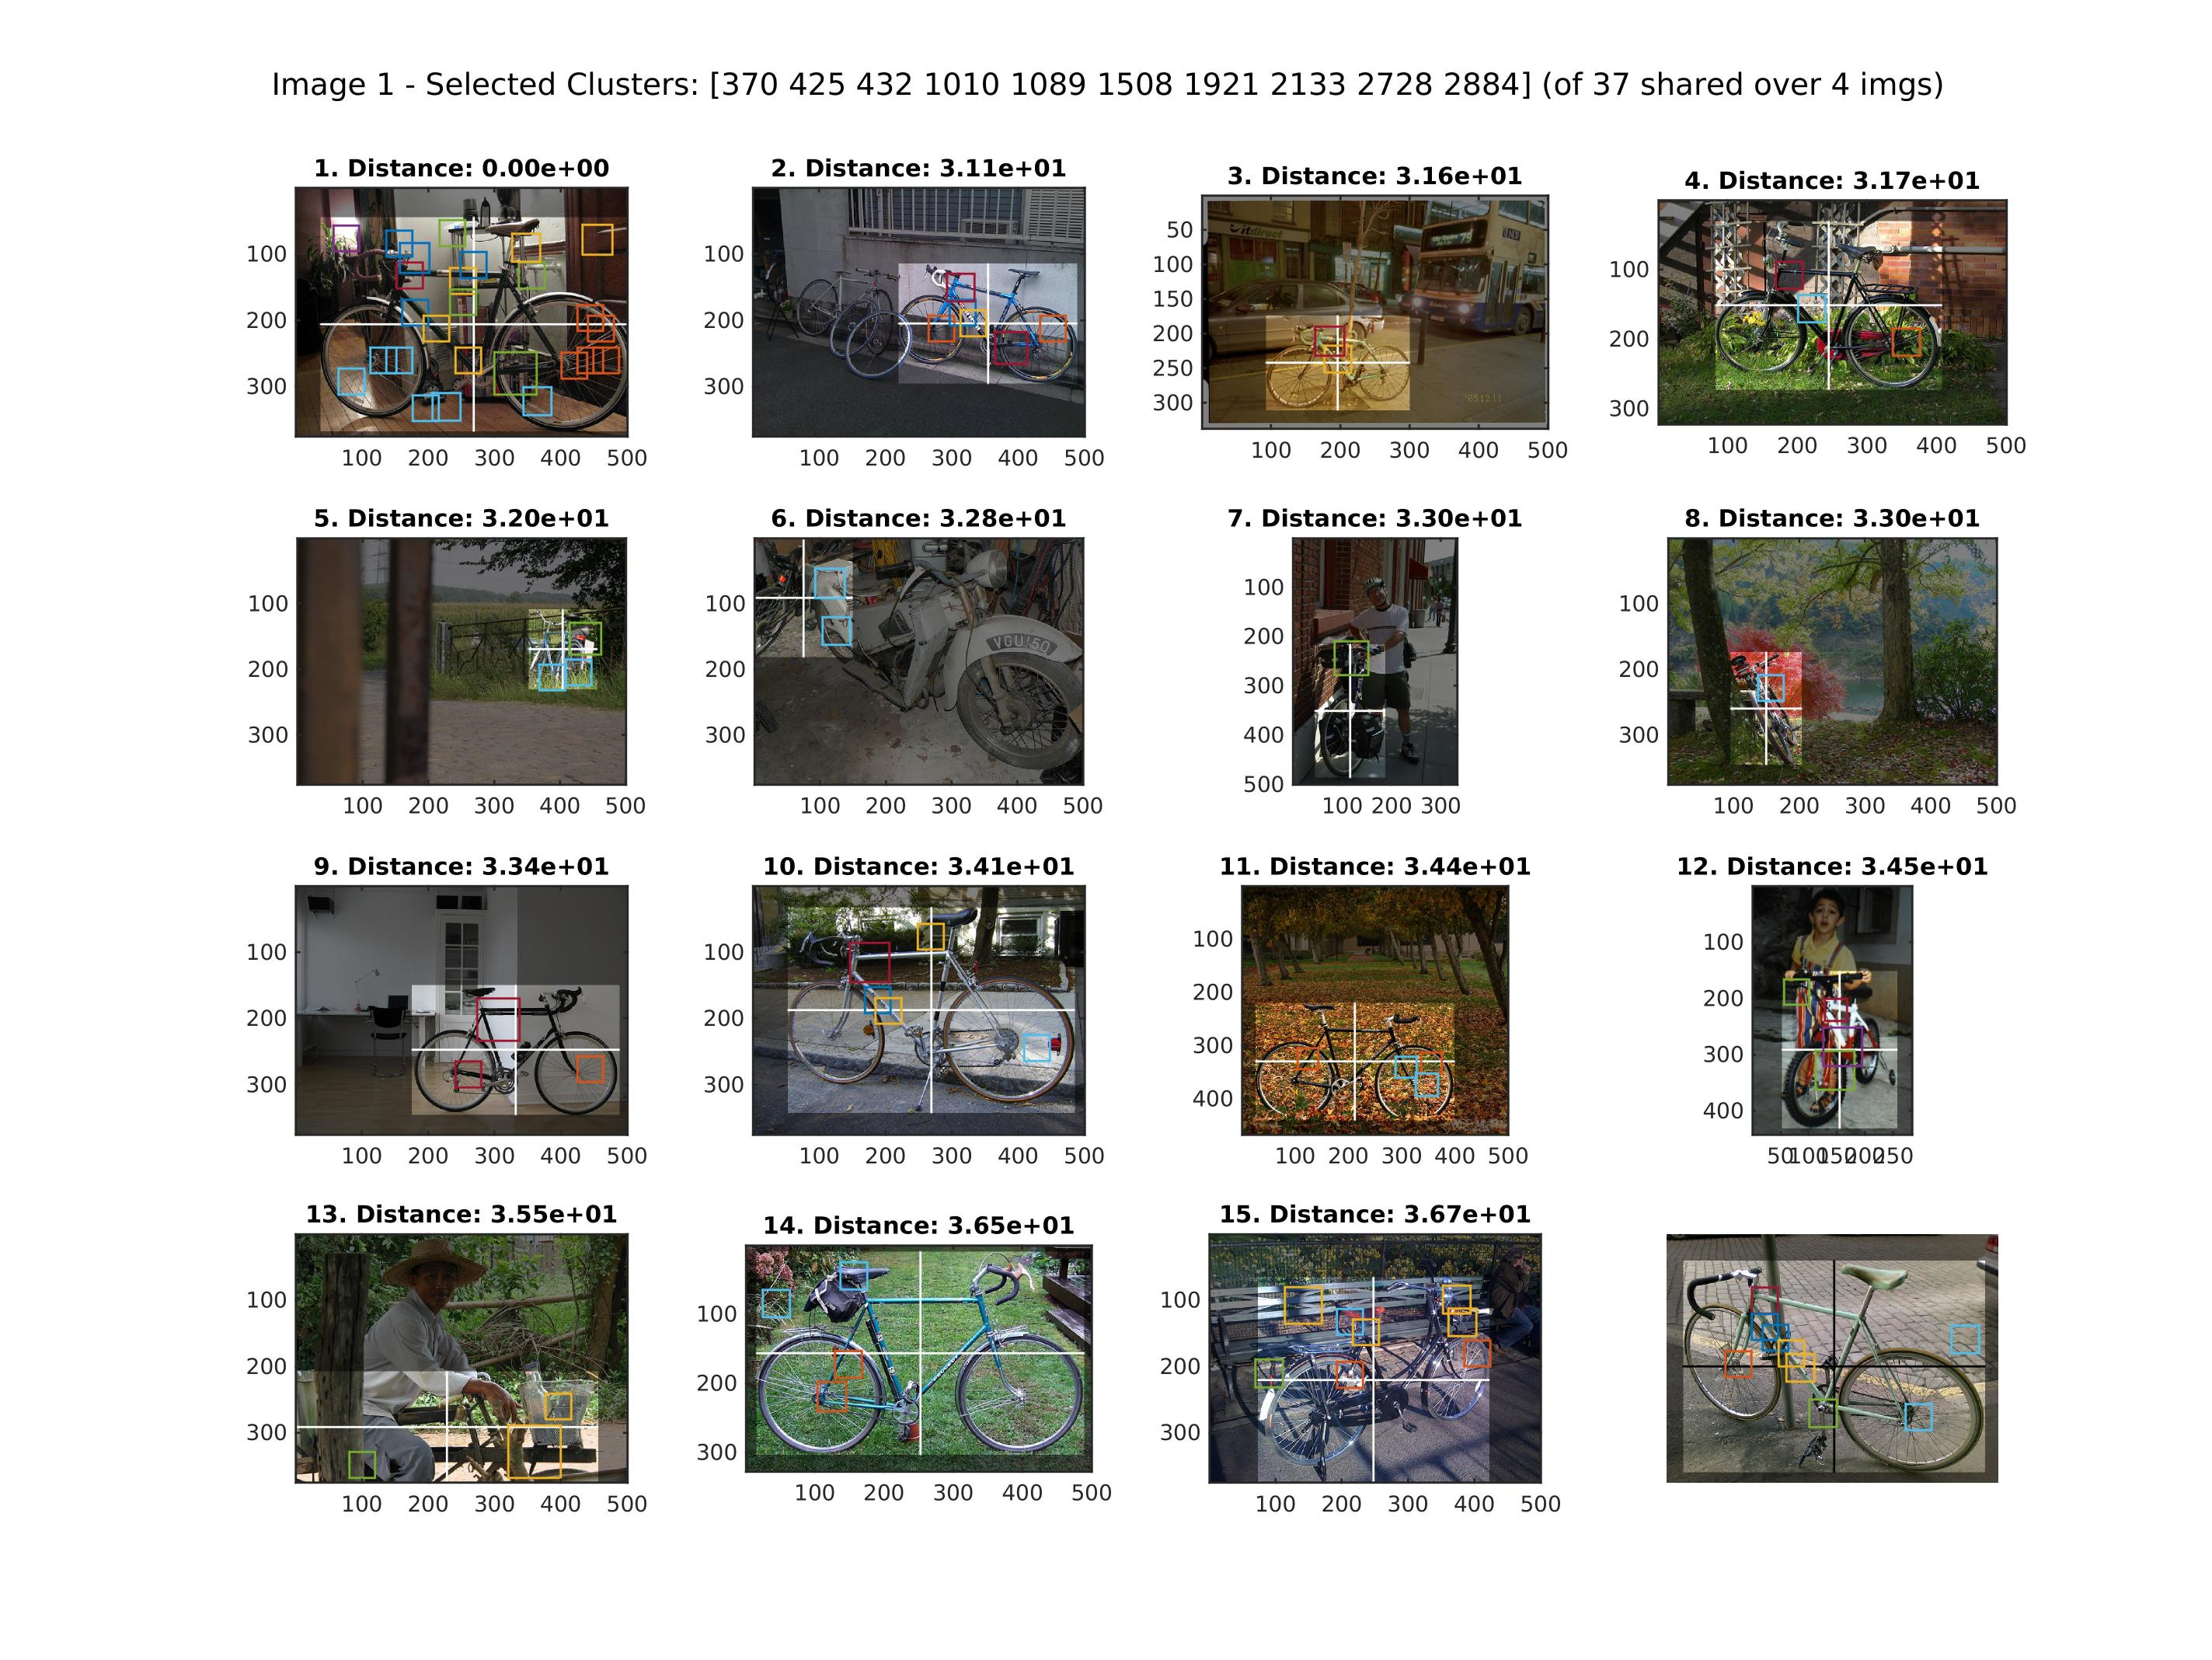
\includegraphics[width=\linewidth]{images/codebook_similiar}
\caption{Comparison of similar images by using codebooks}
\label{fig:nn_query_search}
\end{figure}


After the verification that this approach has the potential to find similar images, further codebook tests were done to get a better feeling of the feature assignments. As the resulting fisher vectors have the size $|x| * k$ (for example with 64 components: $775 * 64 = 49600$) which becomes unusable in terms of memory usage for integral images, they were not further used in favor of the k-means approach.

% searching for representative clusters (nn-iter)
To verify the contribution of the codebook dimensions based on the query, the most shared codebook dimensions within the best 15 remaining images and their respective patches were marked inside the images. It can be clearly seen in \figref{nn_query_search2:common} that the patches with a comparable visual representation share the same cluster and (from a human perspective) seem to be representative for the chosen object class.




To prove this assumption, an iterative \ac{NN} was implemented. It consists of several rounds, each executing a \ac{NN} search over the available patches and sorting the results. After each round, the most common codebook dimensions of the first $k$ patches were taken whilst the remaining ones were removed (set to zero) as described by \prettyref{alg:iterative_nn}.

\begin{algorithm}
	\SetKwProg{Fn}{Function}{}{end}
	\Fn{IterNearestNeighbour($q$ : query codebook, $R$ : remaining codebooks, k)}{
		\Repeat{no changes}{
			$D \gets \text{NearestNeighbourSearch}(R, q)$\;
			
			Sort $R$ based on $D$\;
			
			\tcc{$ij$ denotes dimension $i$ in codebook $j$}
			
			$S = \{i | \forall R_{ij} \ne 0; 0 < j < k\}$\;
			
			$R \gets R_{ij}$ set to $0$ if $i \notin S$\;
		}
		\Return{Sorted $R$}
	}
	\caption{Iterative \ac{NN}}
	\label{alg:iterative_nn}
\end{algorithm}

By using this algorithm, it could be shown that the most representative patches were assigned to the same clusters, as more similar objects are pulled together at each iteration (\figref{nn_query_search2:best}). In nearly all experiments one or two clusters remained which contain patches along the bicycle wheels.



\begin{figure}
\centering
\begin{subfigure}{\textwidth}
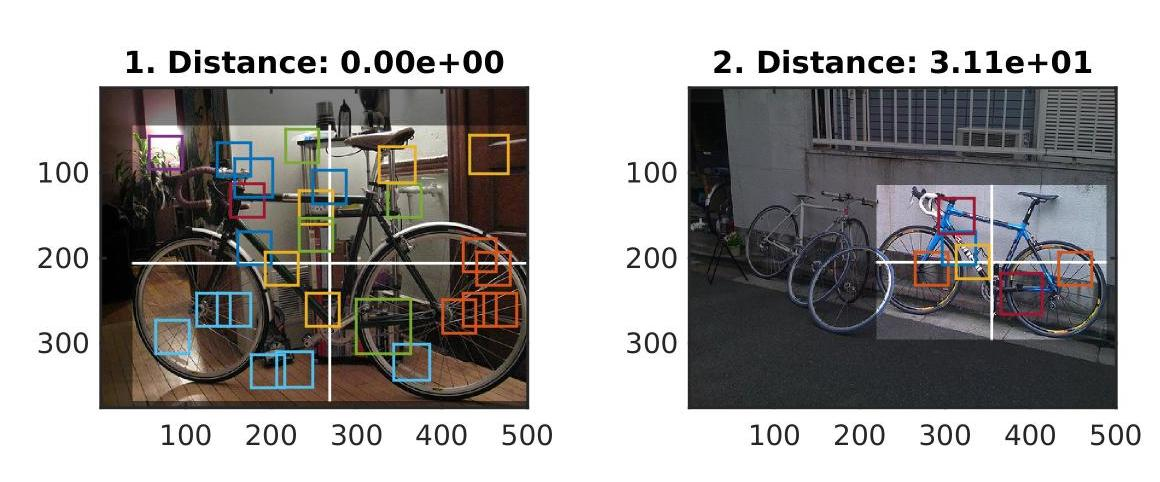
\includegraphics[width=\linewidth]{images/codebook_similiar2}
\caption{Showing common codebook dimensions}
\label{fig:nn_query_search2:common}
\end{subfigure}
\begin{subfigure}{\textwidth}
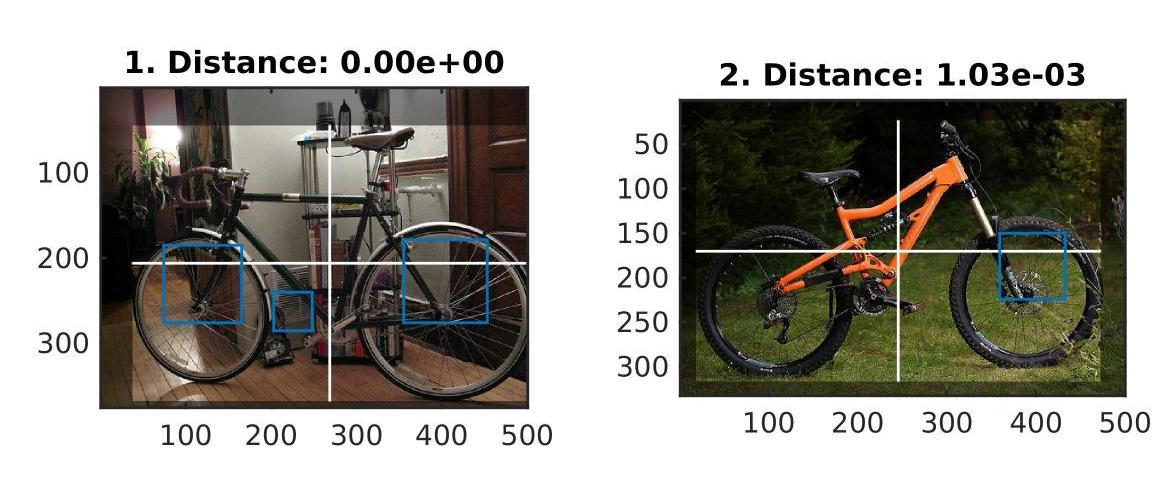
\includegraphics[width=\linewidth]{images/codebook_similiar_best2}
\caption{Showing and using only the most common codebook dimension}
\label{fig:nn_query_search2:best}
\end{subfigure}
\caption{Query part with first detection}
\label{fig:nn_query_search2}
\end{figure}

\par
% maintaining location information (parts)
As the reduction of several feature vectors to a single codebook for a whole bounding box eliminates the locational information, the implementation was extended to maintain some locational information by splitting the bounding box in several parts and computing a codebook for each of them. Afterwards, these codebooks are concatenated, which means that the size of a representative codebook for a whole bounding box is calculated by $numberOfParts * numberOfDimensions$. The number of parts per axis is determined by $round(\sqrt{numberOfParts})$ for the amount of splits in the x direction and $ceil(\sqrt{numberOfParts})$ in the y direction. This change brought additional performance gains in terms of detecting similar parts, but also increased the memory usage and runtime significantly. During the rest of the experiments, the bounding boxes were either split into a two-by-two grid (as it seemed to be the best mix of performance gain and memory usage) or left unsplitted for comparisons.
